\documentclass[a4paper, titlepage]{article}
\usepackage[a4paper,top=2.5cm,bottom=2.5cm,left=3.6cm,right=3.6cm]{geometry}
\usepackage[T1]{fontenc}
\usepackage[utf8]{inputenc}
\usepackage[italian]{babel}
\usepackage{siunitx}
\usepackage{graphicx}
\usepackage{amsmath}
\usepackage{amssymb}
\usepackage{caption}
\usepackage{refstyle}
\usepackage{subfig}
\usepackage{adjustbox}
\usepackage{latexsym}
\usepackage{float}
\usepackage{hyperref}
%
\usepackage{fancyhdr}
\pagestyle{fancy}
\lhead{}
\fancyhead[L]{\leftmark}
\lfoot{}
\cfoot{}
\rfoot{}
\rhead{\thepage}
%
\usepackage{rotating}
\usepackage{booktabs, longtable,afterpage}
\usepackage{rotating}
\usepackage{makecell}
\graphicspath{ {images/} }
\begin{document}
\begin{titlepage}
	\centering
	{\scshape\Large Relazione di laboratorio\par}
	\vspace{0.7 cm}
	\hrule
	\vspace{1.2 cm}
	\begin{figure}[!h]
	    \centering
	    
\includegraphics[width=0.30\textwidth]{Politecnico_di_Torino_-_Logo}
        %\includegraphics[width = 0.50\textwidth]{ITA-template-mesap-01}
	\end{figure}
	
		\vspace{1 cm}
	{\huge\bfseries Rilevamento direzione suono\\ con scheda\\  X-NUCLEO-CCA02M1 \par}
	
	\vspace{2 cm}
	Corso di Laurea Magistrale in Ingegneria Elettronica\par
	\null
	\vfill
	{\raggedright\small Studenti\\\large  Amato Giovanni Luca Matr.267511	\\Cerbai Matilde Matr.274908 \\Chisciotti Laura Matr.274728\\Goti Gianluca Matr.269825\par}
	\vspace{0.2 cm}

	\vfill
	{\large A.A. 2019-20}
\end{titlepage}
\newpage
\tableofcontents
\newpage
\section{Target di progetto}
L'obiettivo di tale progetto è stato determinare la direzione di provenienza di uno schiocco di dita. Per fare ciò è stato necessario l'uso della scheda X-NUCLEO-CCA02M1, per rilevare il suono come flusso PDM, da cui è stato possibile compiere il calcolo dell'energia su due diversi rami e decretare quindi se lo schiocco provenisse da destra, da sinistra o non fosse determinabile la direzione.
\section{Scheda  X-NUCLEO-CCA02M1}
La scheda utilizzata è la X-NUCLEO-CCA02M1. Su questa sono integrati due microfoni MEMS, mediante i quali è stato acquisito lo schiocco in formato PDM, il quale costituisce il punto di partenza su cui si basa l'algoritmo implementato.\\
Tale PDM alterna un bit del microfono destro ad un bit del sinistro.Per fare ciò è infatti necessario che un microfono, nello specifico il destro, campioni sul fronte positivo del clock mentre l'altro, il sinistro, sul fronte negativo.

\section{PDM}
Il PDM, acronimo di "Pulse Density Modulation", è un formato di codifica che permette di rappresentare un segnale analogico, di solito audio, in un un segnale binario adoperando un unico bit. Questo formato  è utilizzabile in tal caso perché garantisce di avere un livello di rumore estremamente più basso e minore interferenza da parte di eventuali segnali.\\Il PDM permette di codificare il segnale sotto analisi, in tal caso uno schiocco, attraverso un solo bit, a differenza del caso PCM ("Pulse Code Modulation"), che invece risulta essere un formato multi-bit.\\Dalla Figura \ref{fig:PDM}, in cui è rappresentato un flusso di PDM, sovrapposto all'andamento di un segnale, è possibile osservare che nei punti in cui l'ampiezza del segnale aumenta, la densità dei PDM con valore 1 è incrementata, mentre là dove il segnale tende a scendere, fino ad arrivare al picco negativo, è presente una maggiore densità dei bit 0.
\begin{figure}[H]
    \centering
    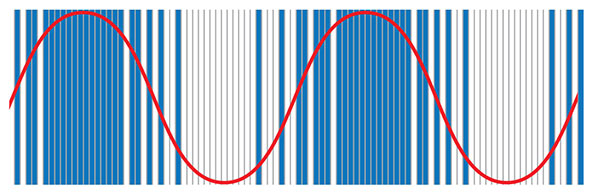
\includegraphics[width=1\textwidth]{PDM.jpg}
    \caption{PDM}
    \label{fig:PDM}
\end{figure}

\noindent Il PDM, utilizzato nel progetto come segnale di ingresso da essere elaborato per determinare la provenienza dello schiocco, è acquisito dai microfoni MEMS della scheda Nucleo ad un'alta frequenza, dell'ordine dei MHz. Questo permette di spostare il rumore in un range di frequenze non udibili dall'orecchio umano, le quali poi verranno eliminate tramite filtraggio.

\section{Double Data Rate (DDR)}
In uscita dalla scheda X-NUCLEO-CCA02M1 è presente un flusso di PDM,che viaggiano su una singola linea sulla quale vengono trasmessi sia i dati del microfono destro che quelli del sinistro in maniera alternata, tale formato é chiamato Double Data Rate (DDR).
La presenza di due informazioni sulla stessa linea é resa possibile inviando il dato relativo al microfono destro sul fronte di salita e quello derivante dal microfono sinistro sul fronte di discesa, tutto avviene in un periodo di clock $T_{clk}$.
Tale processo è visibile in Figura \ref{fig:DDR}, da cui è possibile osservare come, avendo impostato il clock ad una determinata frequenza, in particolare a 2 MHz per quanto riguarda il progetto, il segnale uscente dal microfono destro, cioè il \textbf{PDM\_R} è inviato sul fronte di salita del clock, mentre quello proveniente dal microfono sinistro, \textbf{PDM\_L}, è inviato sul fronte di discesa. L'unione di questi due segnali genera quindi il completo flusso del PDM uscente dalla scheda su una singola linea.

\begin{figure}[H]
    \centering
    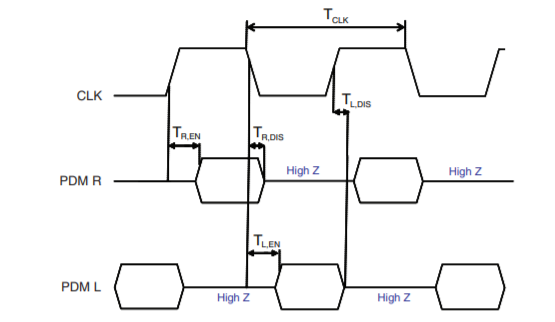
\includegraphics[width=0.8\textwidth]{DDR.PNG}
    \caption{PDM double data rate}
    \label{fig:DDR}
\end{figure}

\section{Flusso di progetto}
Per arrivare alla discriminazione della provenienza dello schiocco, come punto di partenza è stato considerato il flusso PDM provenienti dalla scheda Nucleo, generato a 2 MHz. Questo, contenendo sia l'informazione del microfono destro che sinistro in modo alternato, è stato elaborato in modo tale che le due informazioni venissero smistate rispettivamente sul ramo destro e su quello sinistro. Una volta compiuto ciò, il passaggio successivo è stato quello di andare a ricostruire i campioni del segnale dello schiocco originale, mediante l'utilizzo di un filtro passa basso di tipo FIR ed un sottocampionatore. Quindi, ricavati i campioni ricostruiti, è stato computata l'energia, calcolando in modo sequenziale il quadrato di ciascun campione e poi sommandoli tutti. Questo processo viene attuato per entrambi i rami, in modo da riuscire a decretare l'energia del segnale captato dal microfono destro e quella rilevata dal MEM sinistro. Poi facendo arrivare le energie di entrambi i rami ad un decisore, è stata attuata una discriminazione della provenienza dello schiocco, la quale poi è stata inviata alla UART, in modo tale da trasmettere, secondo il protocollo RS232, il risultato finale al PC, sul cui schermo apparirà S, D o N (Sinistra, Destra o Nullo). 
Tale flusso di progetto è riassunto nello schema in Figura \ref{fig:flusso_progetto}.

\begin{figure}[H]
    \centering
    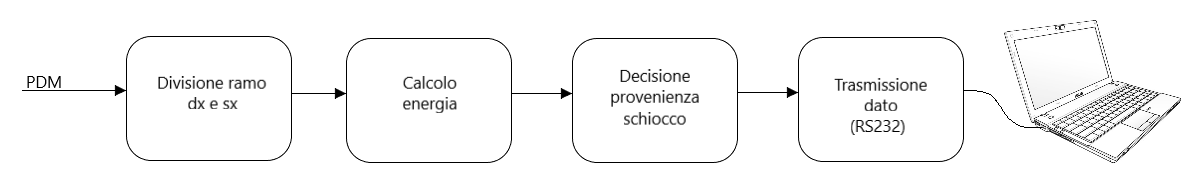
\includegraphics[width=1\textwidth]{flusso_progetto.PNG}
    \caption{Schema flusso di progetto}
    \label{fig:flusso_progetto}
\end{figure}

\section{Filtro passa basso}
\subsection{Cenni di teoria}
All'interno del progetto è stato implementato un filtro passa basso numerico di tipo FIR, cioè "Finite Impulse Response", la cui risposta impulsiva può essere espresso secondo tale formula:

\begin{equation}
y\left [ n \right ]=h_{0}x\left [ n \right ]+h_{1}x\left [ n-1 \right ]+....+h_{N}x\left [ n-N \right ]=\sum_{i=0}^{N}h_{i}x\left [ n-i\right ]
\end{equation}
Per avere una rappresentazione grafica di quanto è stato espresso sopra a livello analitico è possibile riportare il seguente schema a blocchi:

\begin{figure}[H]
\centering
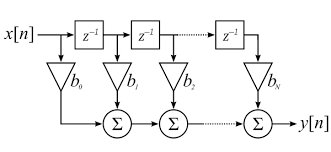
\includegraphics[scale=0.7]{FILTROFIR.png} 
\caption{FIR block diagram}
\label{fig:FIR}
\end{figure}

\noindent Il filtro FIR è un sistema LTI, caratterizzato da una risposta in frequenza di fase lineare e da una risposta impulsiva con un numero finito di campioni. Il suo  ritardo è legato alla sua stessa lunghezza, infatti è importante utilizzare un filtro con ritardo costante poichè nel caso riportato, dopo essere stato progettato, è stato allineato con il dato PDM. Inoltre risulta essere sempre causale e stabile.\\Per realizzare tale sistema è stato utilizzato un Tool di Matlab, che ha permesso di impostare i parametri di progetto scelti.
\subsection{Realizzazione hardware}
%Il blocco "Low Pass Filter", presente nel successivo data path in Figura \ref{fig:BrDP}, è costituito da un filtro passa basso di tipo FIR, che segue la logica di funzionamento spiegata prima teoricamente.\\
Il blocco "Low Pass Filter", presente nel successivo data path in Figura \ref{fig:BrDP}, implementa il filtro descritto in precedenza.
Per quanto riguarda la sua struttura interna, al fine di realizzare la struttura in Figura \ref{fig:LPF}, in VHDL sono stati implementate quattro tipologie di componenti: 

\begin{itemize}
    \item \textbf{shift-register} da 23 %il primo é comb.
    bit, che campiona i bit di PDM in ingresso al filtro, mediante l'enable 1, che arriva dalla CU, dopo che questa è stata stimolata dal segnale in uscita dal primo contatore;
    \item 24 \textbf{coefficienti}, che sono sempre costanti per ogni elaborazione; 
    \item 24 \textbf{moltiplicatori}, che servono per moltiplicare i vari ingressi ritardati con i rispettivi coefficienti;
    \item 23 \textbf{sommatori}, che sommano le uscite dei moltiplicatori.
\end{itemize}
\begin{figure}[H]
\centering
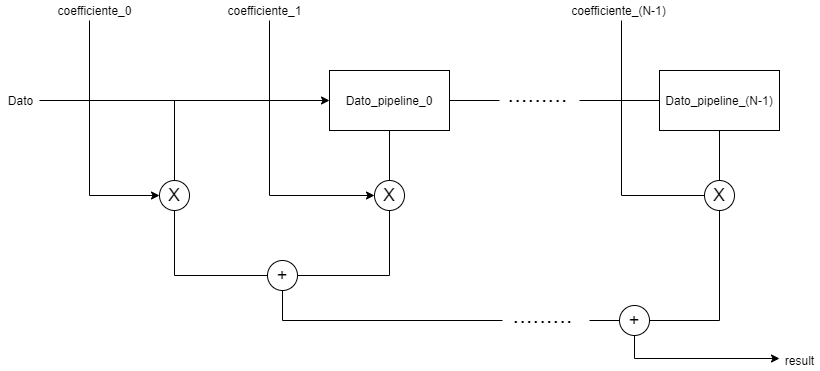
\includegraphics[width=0.8\textwidth]{fir.png} 
\caption{LPF block diagram}
\label{fig:LPF}
\end{figure}
Tale filtro compie una sequenza di moltiplicazioni per i coefficienti e somme, in modo tale da generale i campioni in uscita. 
\subsection{Implementazione filtro}
Il filtro implementato ha un ordine di 23, poichè nel caso in analisi sono necessari 24 coefficienti.\\Per la sua realizzazione è stato fatto uso della funzione Matlab \textbf{firpmord}, che segue l'algoritmo Parks-McClellan, il quale implementa un filtro FIR equiripple.\\La funzione \textbf{firpmord} dà la possibilità di impostare le seguenti specifiche del filtro:

\begin{itemize}
    \item f$_{passband}$=20kHz;
    \item f$_{stopband}$=200kHz;
    \item ampiezza desiderata del ripple;
    \item la frequenza di campionamento f$_{s}$, impostata a 2 MHz.
\end{itemize}

La risposta del filtro ottenuta ha il seguente andamento:

\begin{figure}[H]
    \centering
    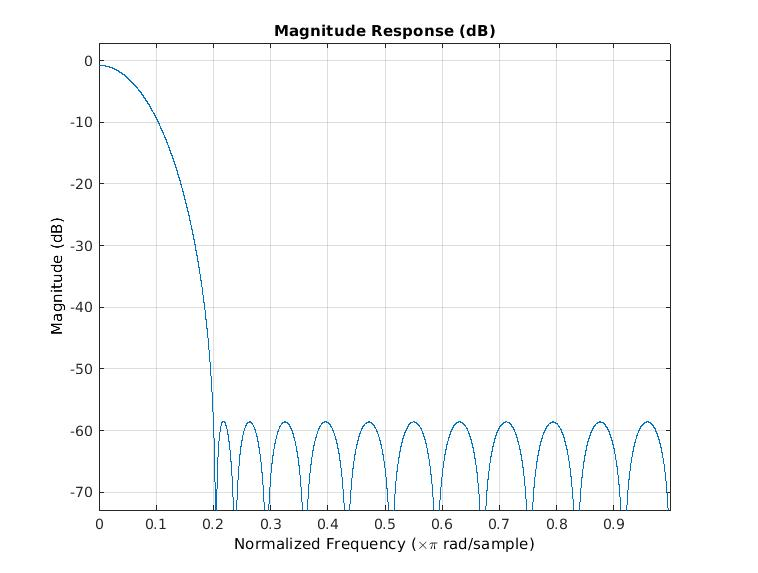
\includegraphics[width=0.8\textwidth]{filtro.jpg}
    \caption{Filtro}
    \label{fig:filter}
\end{figure}

\noindent Da questa immagine è possibile osservare che sulle ascisse le frequenze sono state riportate come normalizzate e per questo assumano tutte valore $\leq$ di 1.\\Successivamente alla realizzazione del filtro, è stata utilizzata la funzione \textbf{firpm}, mediante la quale sono stati estrapolati i coefficienti, i quali sono osservabili dalla risposta impulsiva del filtro, riportata in Figura \ref{fig:risposta impulsiva}, la quale risulta avere una simmetria pari, come è auspicabile aspettarsi dalla teoria del filtro FIR passa-basso.

\begin{figure}[H]
    \centering
    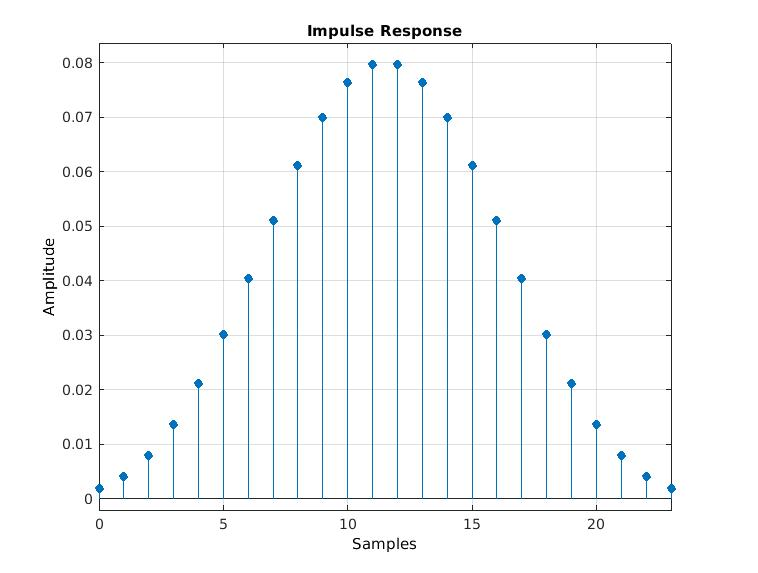
\includegraphics[width=0.65\textwidth]{risposta_impulsiva_filtro.jpg}
    \caption{Risposta impulsiva}
    \label{fig:risposta impulsiva}
\end{figure}

\noindent I coefficienti ottenuti con questa metodologia,  sono poi stati scalati di un fattore dieci, come spiegato nella Sezione \ref{cap:analisi_dati}, per rientrare nella dinamica dei bit di guardia scelti per l'aritmetica interna del sistema. Questi sono stati poi convertiti su 16 bit moltiplicando per un fattore di scala pari a $2^k$ (k=15), in tal modo sono stati ottenuti i seguenti valori dei coefficienti:
\newline
x[n]={7, 14, 27, 45, 70, 100, 133, 168, 201, 230, 251, 262, 262, 251, 230, 201, 168, 133, 100, 70, 45, 27, 14, 7}
\newline
\section{Stima della soglia}
All'interno del blocco decisore, successivamente descritto nella Sezione \ref{cap:data_path}, viene attuata una valutazione dell'energia in ingresso a questo, in modo tale da riuscire a discriminare se tale energia è derivante dal rumore, oppure dal segnale generato dallo schiocco rilevato dai microfoni.\\Per fare ciò è stato necessario impostare una soglia, rispetto alla quale è determinata da cosa deriva l'energia.Infatti se l'energia risulta essere minore od uguale della soglia, questa è associata al rumore, mentre se il suo valore si trova al di sopra della soglia, l'energia è discriminata come derivante dallo schiocco.\\
Quindi la stima della soglia è stata condotta attraverso Matlab, mediante cui è stato implementato un codice che leggesse il file audio .wav dello schiocco, ne estrapolasse lo stream dei PDM e, mediante l'uso del filtro progettato ed attuando un successivo sottocampionamento, sono state poi calcolate le energie dei campioni dello schiocco, il cui stem è riportato in Figura \ref{fig:stem stima soglia}. Da questo è stato decretato un valore intermedio tra quelli più elevati dell'energia. rappresentanti lo schiocco, e quelli più bassi, rappresentanti il rumore. Tale valore corrisponde a E=0,002422.\\Inoltre come conferma ulteriore che tale soglia discriminasse in modo adeguato il rumore, è stato anche mandato in ingresso al codice Matlab un audio contenente solo rumore. Il risultato dell'energia ottenuto da questo è riportato in Figura \ref{fig:stem energia rumore}, da cui si può osservare che rappresentato è corrispondente a 0,0001372 , valore che risulta essere notevolmente inferiore rispetto alla soglia e che conferma quindi la validità della stima condotta.
\begin{figure}[H]
    \centering
    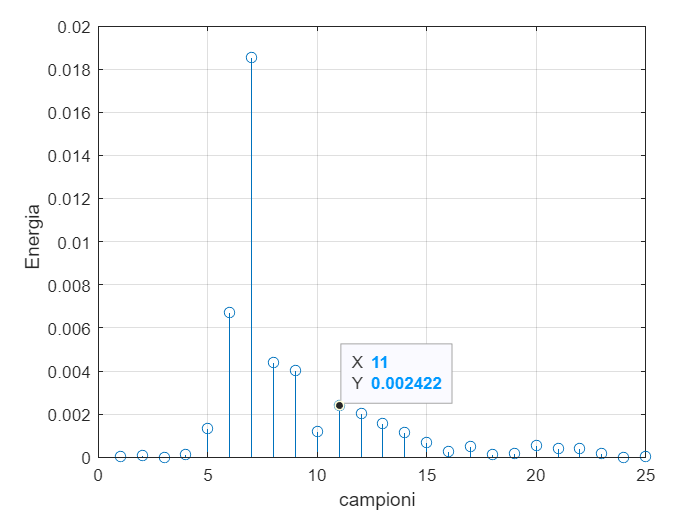
\includegraphics[width=0.8\textwidth]{stem_stima_soglia.PNG}
    \caption{Stem per stima soglia}
    \label{fig:stem stima soglia}
\end{figure}
\begin{figure}[H]
    \centering
    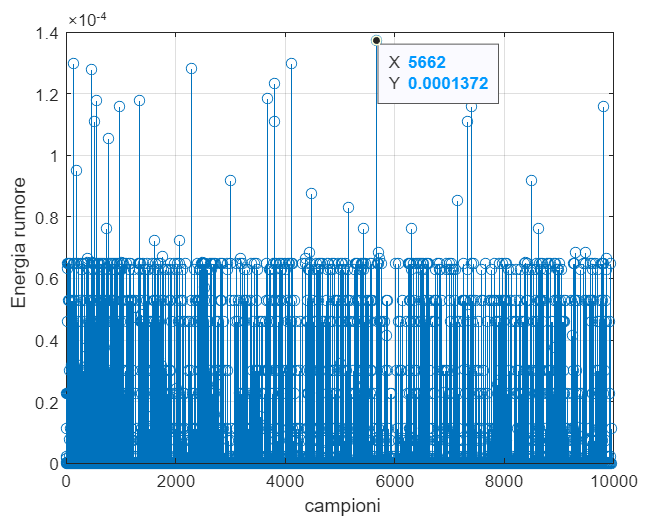
\includegraphics[width=0.8\textwidth]{stem_energia_rumore.PNG}
    \caption{Stem energia del rumore}
    \label{fig:stem energia rumore}
\end{figure}
\section{Data Path}
\label{cap:data_path}
In Figura \ref{fig:DP_completo} è presente il datapath completo della struttura utilizzata per la determinazione da parte dei microfoni della provenienza dello schiocco. Da questa si può osservare che sono presenti due rami, su i quali sono posizionati i blocchi Branch\_1 e Branch\_2. Questi all'interno hanno un'identica struttura, come verrà analizzato in seguito, ma uno è impiegato nel calcolo dell'energia proveniente dal lato sinistro dei microfoni, mentre l'altra dal lato destro.\\Quindi una volta computate le due energie, queste sono mandate all'ingresso del decisore, il quale compie una valutazione della provenienza dello schiocco rilevato, mandando il segnale al multiplexer, il quale invia alla UART il segnale di data valid ed il dato da trasmettere. Inoltre in questo livello gerarchico superiore è anche presente il blocco temporizzatore, impiegato per generare i riferimenti temporali delle diverse operazioni.

\begin{figure}[H]
    \centering
    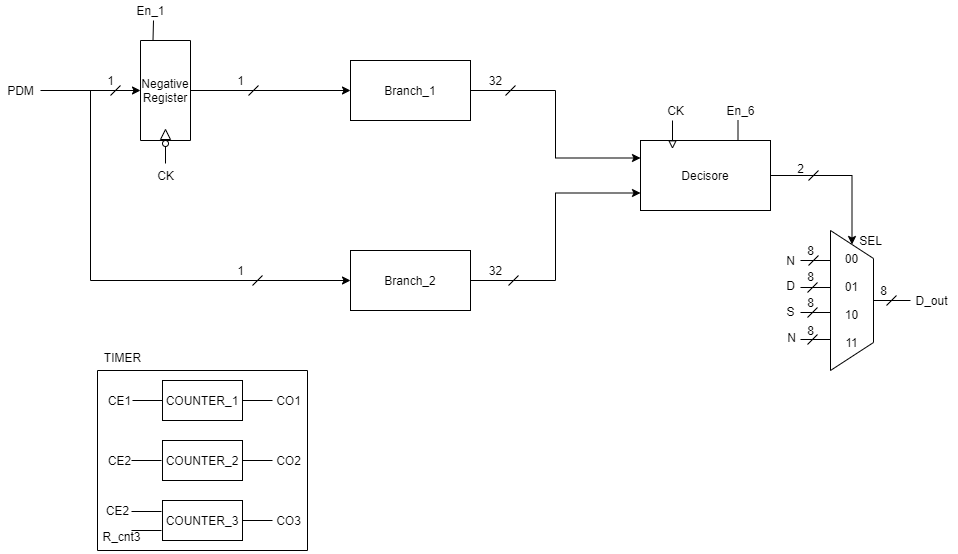
\includegraphics[width=1\textwidth]{DP_completoV2.png}
    \caption{Datapath completo}
    \label{fig:DP_completo}
\end{figure}
\noindent Nella seguente figura è mostrata più nel dettaglio la struttura equivalente dei blocchi Branch\_1 e Branch\_2. Questa è costituita, in modo gerarchico, principalmente dal blocco \textbf{Sign Converter}, che manipola i bit in ingresso provenienti dal PDM, dal blocco \textbf{Low Pass Filter}, da cui escono i campioni ricostruiti del segnale, dal blocco \textbf{Decimatore}, la cui uscita viene moltiplicata per se stessa nel blocco \textbf{Moltiplicatore}, dal blocco \textbf{Sommatore}, che somma dieci campioni, che arrivano in cascata, e dal blocco \textbf{Registro 3}, che rappresenta il registro dell'energia.
\begin{figure}[H]
    \centering
    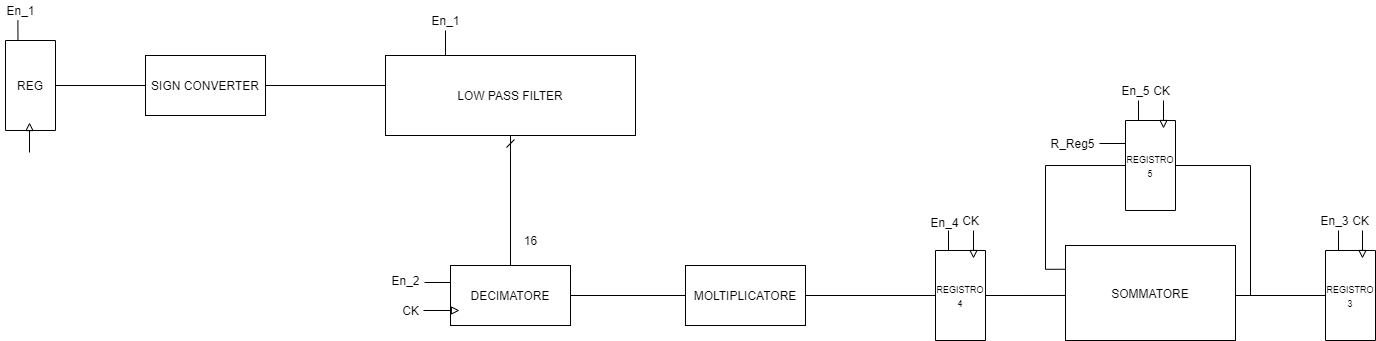
\includegraphics[width=1\textwidth]{Datapath_micV3.png}
    \caption{Branch Datapath}
    \label{fig:BrDP}
\end{figure}
\subsection{Sincronizzazione dei dati in ingresso}
Il metodo di trasmissione dei dati (Double Data Rate) ha imposto l'inserimento di appositi registri per sincronizzare sullo stesso fronte i dati provenienti dai due diversi microfoni. Riferendosi alla Figura \ref{fig:timing_ddr} è possibile osservare che il dato proveniente dal canale sinistro é trasmesso lungo il semi-periodo negativo e il dato proveniente dal canale destro durante quello positivo, questo comporta che il primo deve necessariamente essere campionato sul fronte negativo del clock e il secondo sul fronte positivo, risultando però poi sfasati di mezzo periodo di clock.
\newline
A tal proposito, in ingresso al canale destro è stato inserito un registro attivo sul fronte negativo, in quanto i registri attivi sul fronte positivo sono già presenti in ogni branch per disaccoppiare l'interno della struttura dall'esterno. La struttura "risincronizzatrice" risulta quindi essere come in Figura  \ref{fig:resinc_schematic}, la loro frequenza di lavoro é pari a 
2 MHz, questa é garantita tramite il segnale di enable inviato dalla Control Unit.
\newline
Dal timing si evince che lo sfasamento introdotto dal primo registro é tale per cui il dato campionato dal secondo registro viene sincronizzato con quello proveniente dal secondo microfono, eliminando così lo sfasamento iniziale.

\begin{figure}[H]
    \centering
    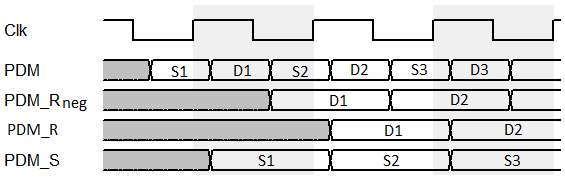
\includegraphics[width=0.8\textwidth]{sincronizzazione_pdm.png}
    \caption{Timing risincronizzazione dei dati PDM}
    \label{fig:timing_ddr}
\end{figure}


\begin{figure}[H]
    \centering
    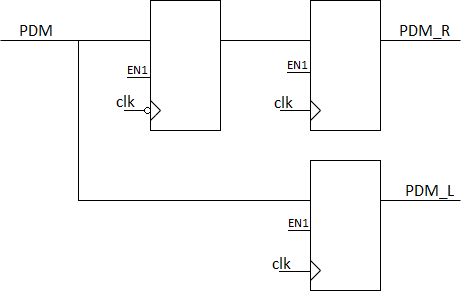
\includegraphics[width=0.5\textwidth]{resinc.png}
    \caption{Circuito risincronizzatore}
    \label{fig:resinc_schematic}
\end{figure}

\subsection{Analisi dei dati}
\label{cap:analisi_dati}
Per tale progetto è stata scelta un'aritmetica fixed point in formato fractional in complemento a due, quindi per definizione del formato la dinamica dei dati é rimasta tra $-1<x<+1$. Per definire il parallelismo dei vari componenti interni al datapath è stata eseguita un'analisi "worst case" dei dati da elaborare.
\newline
Data la natura stessa del PDM i campioni in ingresso al filtro sono valori che assumono solo i valori "+1" e "-1", quindi il caso in cui i dati raggiungono il valore massimo é quello dove tutti i campioni in ingresso al filtro (24 taps) sono pari a "+1" o "-1" e conseguentemente si ha una somma di tutti i coefficienti del filtro.\\ Per semplicità é stato preso in esame il caso con tutti gli ingressi positivi, svolgendo tutti i calcoli previsti all'interno del datapath. E' stato quindi ritenuto necessario l'introduzione di alcuni bit di guardia nei dati in ingresso, così da rispettare il parallelismo scelto e rientrare nella dinamica a disposizione, data la natura degli ingressi, i bit di guardia sono stati utilizzati nei coefficienti del filtro. Quindi, scalando di un fattore dieci i valori ottenuti dallo script Matlab, é stato possibile ridurre la dinamica dei coefficienti stessi, ottenendo così un numero di bit di guardia pari a 6 (la dinamica deve essere $|x|<\dfrac{1}{2^6}$ e infatti il massimo valore é 0,008).\\ Le moltiplicazioni all'interno del filtro non hanno particolari problemi in quanto sono presenti solamente somme e sottrazioni tra coefficienti e questo non ha modificato il parallelismo dei dati in uscita che é rimasto pari a 16 bit. %Questo però é aumentato dopo il blocco moltiplicatore arrivando a 32 bit. 
Quindi, nel caso peggiore all'uscita del filtro è presente un numero pari a $\simeq 0,0092$. Questo é ancora rappresentabile su 16 bit in quanto usando il fattore di scala $2^k$ (k=15) e riconvertendolo con esso, si ottiene $0,0092*2^{15}\simeq3016$, che é minore del massimo numero rappresentabile su tale numero di bit.
\newline
In uscita dal moltiplicatore è stato adottato un parallelismo doppio (32 bit) in quanto una moltiplicazione in formato fractional su "n" bit rende "2n" bit.\\ L'ultima operazione richiesta é una somma delle energie relative a 10 campioni, moltiplicando per due il dato in uscita dal moltiplicatore per eliminare il segno raddoppiato che si produce nell'operazione di moltiplicazione e sommando dieci volte il risultato ottenuto, è stato ricavato un valore pari a $(0,0092)^2*2*10\simeq0,169$, che rimane nella dinamica necessaria, quindi anche il sommatore é stato progettato con parallelismo pari a 32 bit ($0,169*2^{31}=363850240$ é minore del massimo numero rappresentabile con tale numero di bit). E' stato deciso quindi di optare nel mantenimento di un parallelismo doppio dopo il moltiplicatore, così da avere una precisione maggiore sui risultati. Quindi, ricapitolando sono stati adottati:
\begin{itemize}
    \item [--] 16 bit per filtro e decimatore;
    \item [--] 32 bit per moltiplicatore e sommatore.
\end{itemize}


\subsection{Descrizione dei componenti}
\subsubsection{\textbf{Branch}}
I dati in ingresso a tale blocco sono campionati da un apposito registro operante a 2MHz che ha sia la funzione di disaccoppiare i dati provenienti dall'esterno all'interno del sistema, sia quello di sincronizzare, con l'aggiunta di un registro attivo sul fronte negativo in uno dei due rami, i dati provenienti dai due microfoni nei rispettivi canali. I restanti componenti sono descritti di seguito.
\begin{itemize}
    \item [--] \textbf{Sign converter}
    \newline
    Come detto in precedenza i dati in ingresso sono solo "+1" e "-1", i quali però sono codificati rispettivamente su "1" e "0". A tal proposito è stato progettato il blocco Sign Converter, in modo da trasformare i dati binari nei dati corretti su un formato di 16 bit, adottando così un parallelismo uguale ai coefficienti del filtro.
    \item [--] \textbf{Decimatore}
    \newline
    I dati in uscita dal filtro hanno una frequenza pari a 2MHz per ricostruire i dati in PCM é stato necessario sottocampionarli riportandosi ad una frequenza pari a 40 KHz, mediante un decimatore, composto semplicemente da un registro.\\Va posta particolare attenzione sui dati in uscita dal filtro, questi hanno un parallelismo pari a 32 bit, in quanto vi sono moltiplicazioni tra dati su n bit che rendono un risultato su 2n bit. Analizzando però con più attenzione i dati in possesso, è stato possibile notare che anche nel caso peggiore, ovvero quello in cui vengono sommati tutti i coefficienti, il risultato rimane su 16 bit (la metà inferiore dei 32 bit), per questo la metà superiore del dato é inutilizzata. E' questo il motivo per cui a livello VHDL è stato scelto di riportare il dato su 16 bit, in quanto tale operazione non comporta una perdita di precisione sul risultato. Per compiere ciò é stato eseguito uno shift left di 16 posizioni del risultato in uscita dal filtro ed in seguito è stato compiuto un taglio per selezionare i 16 bit più significativi.
    \item [--] \textbf{Moltiplicatore}
    \newline
    Questo blocco esegue la moltiplicazione per calcolare il quadrato dei coefficienti della sequenza filtrata in ingresso, essendo anche questa una moltiplicazione su 16 bit ed essendo il risultato su 32 bit, è stato necessario eseguire uno shift left per eliminare il segno raddoppiato dall'operazione di moltiplicazione (é stata usata la libreria numeric\_std).
    \newline 
    Per immagazzinare il risultato di tale operazione e renderla stabile per le seguenti elaborazioni, é stato inserito un registro munito di enable.
    \item [--] \textbf{Sommatore}
    \newline
    Per completare il calcolo dell'energia sono stati sommati i quadrati dei campioni filtrati, progettando una struttura con un sommatore ed un registro in retroazione. Tale registro é necessario in quanto le somme avvengono solamente ad una frequenza pari a
    40 KHz, quindi è necessario mantenere il risultato calcolato al passo precedente.\\ Il registro che permette di fare la ricorsione ha un reset asincrono, che garantisce la possibilità di azzerare il contenuto dello stesso.\\ Come detto in precedenza, i bit di guardia permettono di rimanere nei 32 bit senza bisogno di prevedere l'utilizzo di bit in più per sopperire ad eventuali overflow.
    
     \item [--] \textbf{Registro energia}
     In uscita al sommatore è stato posto un registro dotato di enable, il quale è attivato con timing opportuno per prendere l'energia corrispondente a 10 campioni.
    \newline
\end{itemize}
\subsubsection{\textbf{Datapath}}
Al livello gerarchico superiore sono state istanziate due versioni del componente "branch" una per il canale destro e una per il canale sinistro, com'è osservabile in Figura \ref{fig:DP_completo}. In ingresso al branch destro è stato inserito il flip-flop attivo sul fronte negativo per attuare la risincronizzazione del PDM proveniente dal microfono destro.
I blocchi principali sono: 
\newline
\begin{itemize}
    \item [--] \textbf{Decision Maker}
        Questo é uno dei blocchi più importanti dell'intero sistema, analizza le energie derivanti dal processo di filtraggio e di somma e le confronta con una soglia. 
        \newline
        Internamente vi é un comparatore che valuta le energie di entrambi i canali per vedere quale delle due é maggiore, una volta assicurato ciò si compara l'energia "vincitrice" con la soglia, questo porta ad "1" uno dei due segnali segnali i quali poi vengono mandati in ingresso ad uno shift register opportunamente pilotato.
        Le uscite parallele dello shift register di dimensione pari a quattro sono mandate ad un majority voter che riconosce se ci sono tre o più elementi ad "1". Questa condizione é stata ritenuta necessaria e sufficiente a rilevare uno schiocco, in termini temporali tutto ciò corrisponde ad avere per 750 $\mu$s un'energia sopra la soglia e quindi uno schiocco (l'energia é valutata in slot da 250 $\mu$s); non é stata scelta una condizione con quattro "1" in quanto é stata ritenuta troppo stringente. I due bit (segnale DCN) uscenti dal majority voter sono mandati alla control unit.
        In Figura \ref{fig:decisore_schematic} é riportato lo schema di principio del decisore.
        
        \begin{figure}[H]
        \centering
        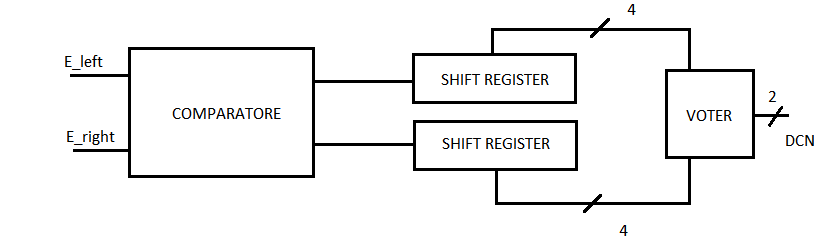
\includegraphics[width=0.8\textwidth]{decisore.png}
        \caption{Schema a blocchi del decisore}
        \label{fig:decisore_schematic}
        \end{figure}
        
    \item [--] \textbf{Mux}
    \newline
    Il mux ha il compito di porre il carattere ASCII corretto in ingresso alla porta D\_out della UART, viene girato dalla Control Unit che reagisce agli stimoli inviati dal segnale DCN proveniente dal blocco decisore.
    \item [--] \textbf{Timer}
    \newline
    Questo elemento gestisce la temporizzazione di tutto il sistema. Al suo interno si trovano tre contatori:
    \begin{itemize}
        \item Contatore 1:
        \newline
        gestisce tutta la temporizzazione in ingresso del segnale PDM, alla scheda. E' fornito un clock di 2 MHz, quindi questo contatore genera tutti gli enable per gestire i registri ed il filtro con la medesima temporizzazione;
        \item Contatore 2:
        \newline
        questo contatore si occupa di generare l'enable per attivare il decimatore con una frequenza di 40 kHz. Infatti per riuscire a fare ciò il contatore è stato progettato per contare da 0 a 49, cioè 50, fattore ricavato dalla divisione $\frac{2 MHz}{40 kHz}$;
        \item Contatore 3:
        \newline
        l'ultimo contatore permette di gestire le dieci somme per calcolare l'energia sui dieci campioni. Questo é stato fatto contare da 0 a 8 (contando quindi fino a 9) generando così la condizione di uscita nella macchina a stati per proseguire l'evoluzione degli stati. Anche per questo motivo tale contatore ha un reset sincrono che viene attivato una volta avvenuta la condizione citata in precedenza.
    \end{itemize}
    
\end{itemize}

\subsubsection{\textbf{Top Level}}
All'ultimo livello gerarchico è stata inclusa anche la UART per inviare i dati all'esterno. Alla porta di ingresso D\_out é collegata l'uscita del mux in modo da inviare la word corrispondente alla rilevazione effettuata. Il Data\_valid é fornito dalla Control Unit e il Tx\_rdy é mandato alla stessa per verificare l'effettiva disponibilità del trasmettitore ad inviare la word sul bus.
\section{Control Unit}
La Control Unit (CU) impiegata per questo progetto è composta da una parte sequenziale, che fa progredire gli stati e compiere salti dove è necessario, ed una parte puramente combinatoria, che ha il compito di mandare i comandi al data path. La struttura di tale CU è osservabile in Figura \ref{fig:CU_struttura}, da cui è possibile notare la presenza di un registro all'uscita del bloccho "next state logic", impiegato per svincolarsi dall'esterno ed evitare la creazione di una macchina di Mealy. 
\begin{figure}[H]
    \centering
    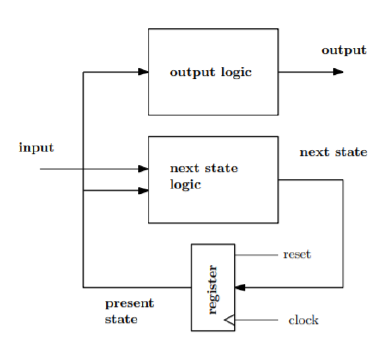
\includegraphics[width=0.6\textwidth]{CU_struttura.png}
    \caption{Struttura control unit}
    \label{fig:CU_struttura}
\end{figure}
\noindent Il flusso specifico di funzionamento della CU in questione è raffigurato in Figura \ref{fig:pallogramma}.
\begin{figure}[H]
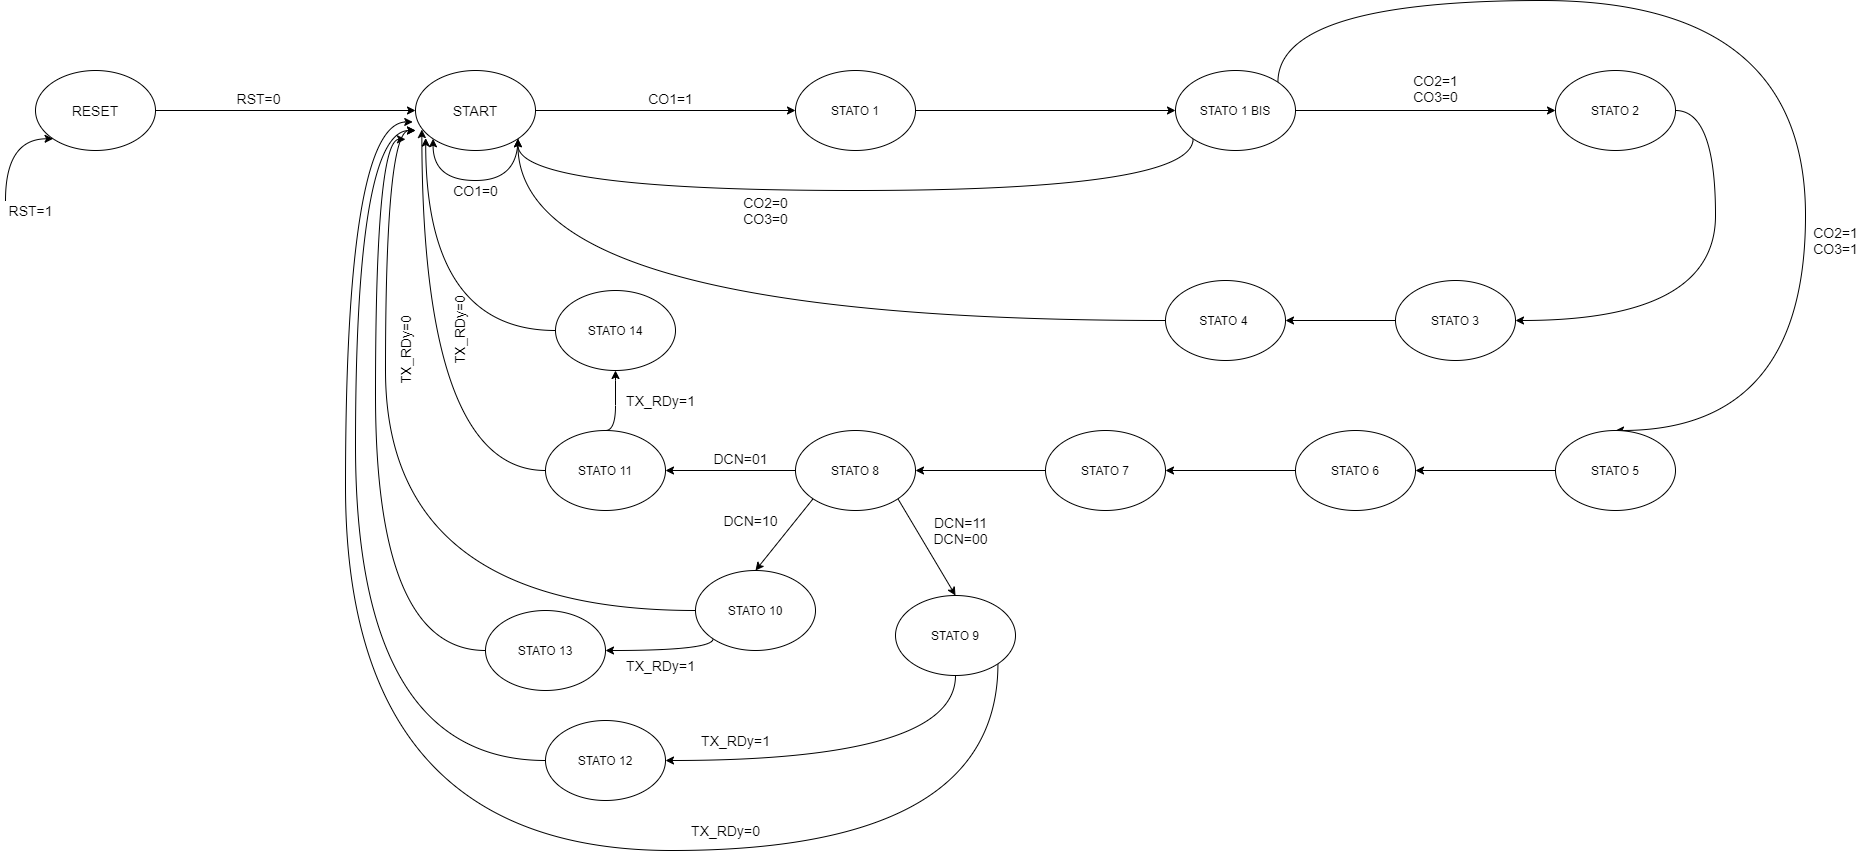
\includegraphics[width=1\textwidth]{Palleogramma_micV2.png}
    \caption{Pallogramma}
    \label{fig:pallogramma}
\end{figure}

\noindent Quando il segnale RST è a zero, dallo stato di "RESET", si salta in "START", in cui viene attivato il primo contatore, che rileva i bit di PDM che arrivano all'ingresso dei microfoni. Da questo stato poi si passerà a "STATO\_1" se il segnale CO1 è asserito ad 1, altrimenti si resta nello stato attuale. Nello "STATO\_1" viene alzato l'En\_1, il quale va a comandare sia i registri del double data rate, sia il primo shift register di ciascun branch. Inoltre in questo stato viene anche attivato il secondo contatore, il quale conta 50 PDM. Quindi da qui in modo sequenziale si passa allo "STATO\_1\_BIS", in cui si ha un salto a tre vie, ovvero se CO2=0 e CO3=0 si torna in "START", poiché il secondo e il terzo contatore non hanno terminato di contare e quindi ciclicamente è necessario ripercorrere gli stati precedenti, se CO2=1 e CO3=0 indica che il secondo contatore ha terminato di contare e quindi è possibile ricavare il primo campione dal decimatore, quindi si passa allo "STATO\_2" oppure se CO2=1 e CO3=1 significa che sia il contatore 2 che 3 hanno terminato il conteggio, ovvero è possibile estrapolare il primo valore dell'energia, e quindi si salta allo "STATO\_5".\\Riposizionandosi sullo "STATO\_2", da qui si procede in modo sequenziale allo "STATO\_3" e "STATO\_4", per poi tornare a "START".\\Ponendosi invece sullo "STATO\_5", si procede anche qui in sequenza, fino allo "STATO\_8".\\In questo è presente nuovamente un salto a tre vie, comandato dal segnale DCN, il quale è composta da due bit e porta allo "STATO\_9" se asserito al valore "11" o "00", in cui il selettore del multiplexer in uscita dal datapath gira il mux sulla codifica ASCII di N, oppure allo "STATO\_10" se il suo valore è "10", in cui il SEL assume la codifica "10", mandando in uscita la D, altrimenti se DCN="01" va allo "STATO\_11", in cui SEL="01" e il mux si gira sulla codifica della lettera S.\\ Quindi da ciascuno di questi tre stati è possibile percorrere due strade ovvero:
\begin{itemize}
\item se TX\_RDY='1', cioè il trasmettitore è libero ed è permesso l'invio di un dato, c'è un salto sullo "STATO\_12", in cui viene mantenuto il SEL="11" 0 "00" ed il D\_valid viene asserito alto, se precedentemente si era nello "STATO\_9", oppure nello "STATO\_13", dove il SEL resta a "10" e si attiva il D\_valid, se il sistema era nello "STATO\_10", altrimenti se lo stato precedente era lo "STATO\_11", il salto viene compiuto sullo "STAO\_14", in cui il SEL vale ancora "01" ed il D\_Valid va all'uno logico. Il fatto di alzare il D\_valid, comporta l'invio del dato alla UART;
\item se TX\_RDY='0', cioè il trasmettitore è "busy", perché sta già trasmettendo un dato, allora il salto, da ciascuno dei tre stati, viene fatto direttamente sullo stato di "START".
\end{itemize}
\section{Timing}
Il timing è stato analizzato suddividendolo in due parti: una che si concentra sul comportamento del branch e del decisore  ed una che analizza più nello specifico la parte di invio del dato al trasmettitore mediante il multiplexer.
\subsection{Timing branch \& decisore}
In questa parte è analizzato il timing riguardante il branch ed il decisore, ovvero la parte della struttura in cui viene calcolata l'energia e la parte che confronta le energie dei due rami, valutando la direzione di arrivo dello schiocco.\\I segnali utilizzati, com'è osservabile in Figura \ref{TX Timing}, sono i seguenti:
\begin{itemize}
    \item \textbf{CLOCK}: clock a 25 MHz; 
    \item \textbf{PDM}: segnale a 2 MHz in ingresso al datapath, che viene smistato al ramo destro e sinistro mediante i regitri del double data rate;
    \item \textbf{CE1}: counter enable del COUNTER 1;
    \item \textbf{CO1}: segnale che indica che il primo contatore ha terminato di contare;
    \item \textbf{En\_1}: segnale di enable dello shift register da 24 bit;
    \item \textbf{CE2}: counter enable del COUNTER 2;
    \item \textbf{CO2}: segnale di termine conteggio del secondo contatore;
    \item \textbf{En\_2}: segnale di enable del decimatore; 
    \item \textbf{En\_4}: segnale di enable del registro tra il moltiplicatore ed il sommatore;
    \item \textbf{En\_5}:segnale di enable del registro di retroazione al sommatore;
    \item \textbf{CE3}: counter enable del COUNTER 3;
    \item \textbf{CO3}: segnale che indica quando il terzo contatore ha finito di contare;
    \item \textbf{En\_3}: segnale di enable del registro dell'energia; 
    \item \textbf{R\_cnt3}: segnale di reset del terzo contatore;
    \item \textbf{R\_reg5}: segnale di reset del registro ;
    \item \textbf{En\_6}: segnale di enable del decisore ;
    \item \textbf{RST}: reset del sistema.
\end{itemize}

Dalla figura del timing è possibile analizzare come avviene tutto il processo di calcolo dell'energia, il quale parte dal momento in cui, accendendo i microfoni, si asserisce a livello logico alto il CE1, che rimane ad 1 fino a quando non viene spento il sistema o finché non arriva il segnale di reset generale del sistema.\\ Una volta quindi che il CE1 risulta essere all'uno logico, il contatore 1, che conta 13 colpi di clock, corrispettivi ad un PDM (questa é un'approssimazione in quanto il numero esatto sarebbe 12,5), si accende. Ogni volta che il COUNTER 1 termina di contare, ovvero quando è entrato nel sistema un intero PDM, viene asserito ad 1, per un solo colpo di clock, il segnale CO1. Questo andando alla control unit, va a stimolare l'invio da questa dell'En\_1, che va ad attivare sia il registro che campiona sul fronte negativo, sia il registro che campiona sul fronte positivo, posizionato subito prima dello shift register da 24 bit, sia lo shift register stesso. \\In concomitanza dell'En\_1, viene portato ad 1, per un colpo di clock, il segnale CE2, che va ad attivare il secondo contatore. Tale processo viene reiterato per 50 volte, dato che tale valore corrisponde al fattore di sottocampionamento utilizzato dal decimatore. Arrivata la cinquantesima volta in cui viene asserito CE2, al colpo di clock successivo viene alzato per CO2, che arrivando alla CU, indica che il secondo contatore ha terminato di contare e che il decimatore può essere abilitato. Quindi la CU invia a questo il segnale di En\_2, che dura anch'esso un singolo colpo di clock. In cascata a tale enable vengono asseriti a livello logico alto anche l'En\_4, che attiva il registro di memorizzazione del dato in uscita dal moltiplicatore, e successivamente l'En\_5, che abilita il registro presente sulla retroazione del sommatore.\\In corrispondenza temporale dell'En\_2, è presente anche l'asserimento ad 1 del CE3, per un solo colpo di clock ogni volta. Questo va ad attivare il terzo contatore, che non va a contare un numero di colpi di clock, ma conteggia per nove volte l'En\_2. Quindi il processo fin'ora spiegato viene implementato per 9 volte, per poi asserire, al colpo di clock successivo alla nona volta che CE3 va ad 1, il segnale CO3 a livello logico alto. Questo resterà alto finché dalla control unit non arriverà il segnale R\_reg5, che resetta il terzo contatore.\\Successivamente per la decima volta viene iterato il processo descritto, con la differenza che ora il CO3 è alto. E' proprio tale fattore che permette di avere una condizione che permetta di resettare il terzo contatore e quindi di abbassare il segnale CO3. Infatti nell'ultima parte di timing è possibile osservare che in un punto viene soddisfatta la condizione di avere C2=1 e CO3=1, il quale consegue di avere, due colpi di clock dopo, l'asserimento a livello alto di R\_cnt3, che, mandato dalla CU, arriva al COUNTER 3, resettandolo.\\Ciò comporta quindi un abbassamento di CO3 e l'abilitazione dell'En\_3, il quale va ad abilitare il registro che memorizza l'energia calcolata. Poi un colpo di clock successivo ad En\_3 viene compiuto l'asserimento ad 1 del segnale R\_Reg5, che va a resettare il registro sulla retroazione del sommatore, il quale memorizza il risultato in uscita dal sommatore e lo va a far sommare all'ingresso successivo.\\Il timing fin qui descritto vale sia per il ramo destro che per quello sinistro, compiendo simmetricamente le stesse azioni.
Successivamente dai due rami delle energie, il sistema convoglia nel decisore, il quale è controllato dall'En\_6, che si attiva un colpo di clock dopo l'enable del registro dell'energia. Da tale decisore uscirà quindi il segnale di DCN, il quale assume un valore differente a seconda del risultato della valutazione dell'energia ottenuta.

\begin{sidewaysfigure}
\centering
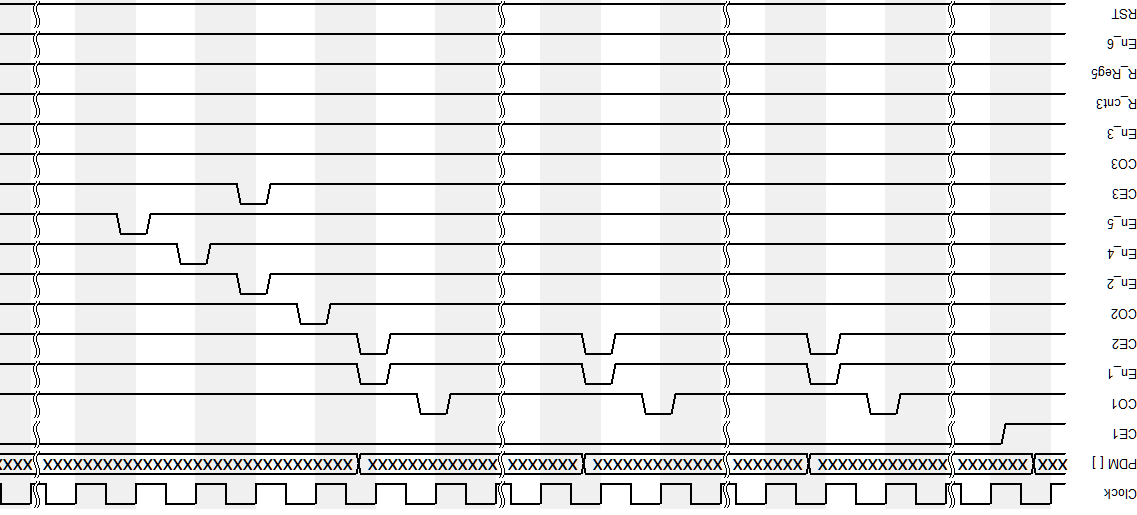
\includegraphics[scale=0.7]{timingmicV3_1.png} 
\caption{Timing}
\label{TX Timing}
\end{sidewaysfigure}
\begin{sidewaysfigure}
\centering
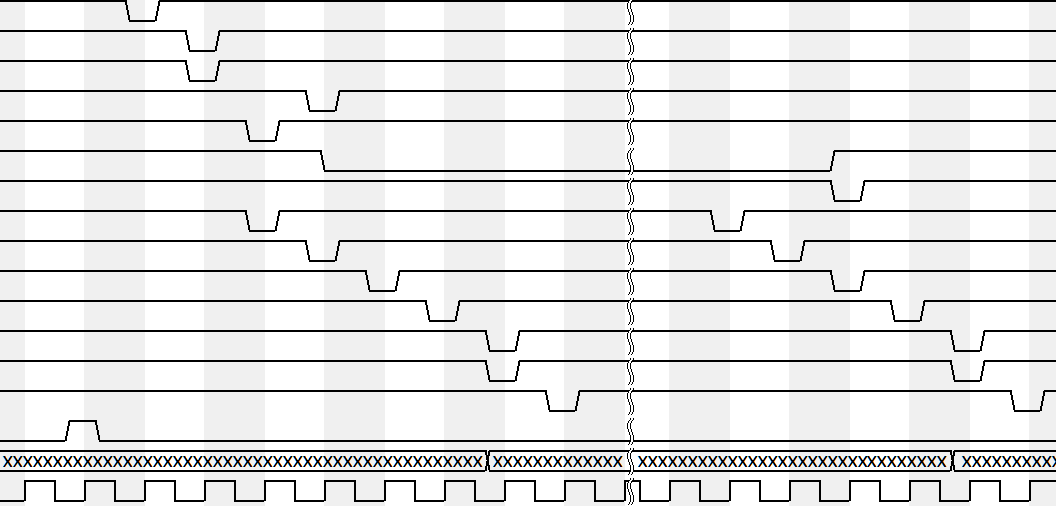
\includegraphics[scale=0.7]{timingmicV3_2.png} 
\end{sidewaysfigure}
\newpage
\subsection{Timing invio dato al trasmettitore}
In Figura \ref{fig:timing_small} è presente il timing che mostra l'invio del dato in uscita dal multiplexer, al trasmettitore. A seconda del valore che assume il selettore, il mux viene girato, mandando in uscita le seguenti codifiche binarie su 8 bit:
\begin{itemize}
    \item se SEL="00" oppure SEL="11" $\longrightarrow$ D\_out="01001110", che corrisponde alla codifica ASCII della lettera N, se la provenienza dello schiocco non è identificabile;
    \item se SEL="01" $\longrightarrow$ D\_out="01000100", che corrisponde alla codifica ASCII della lettera D, se lo schiocco proviene da destra;
    \item se SEL="10" $\longrightarrow$ D\_out="01010011", che corrisponde alla codifica ASCII della lettera S, se lo schiocco proviene da sinistra.
\end{itemize}
Tale timing è caratterizzato dai seguenti segnali:
\begin{itemize}
    \item \textbf{CLOCK}: clock a 25 MHz; 
    \item \textbf{DCN}: segnale da due bit in uscita dal decisore;
    \item \textbf{SEL}: segnale da due bit in ingresso al multiplexer;
    \item \textbf{TX\_RDY}: segnale inviato dal trasmettitore per indicare se esso stesso è "busy", oppure se è libero per potergli inviare un dato da trasmettere;
    \item \textbf{D\_valid}: segnale di invio del dato;
    \item \textbf{D\_out}: dato che viene inviato in uscita dal mux.
\end{itemize}
\begin{figure}[H]
    \centering
    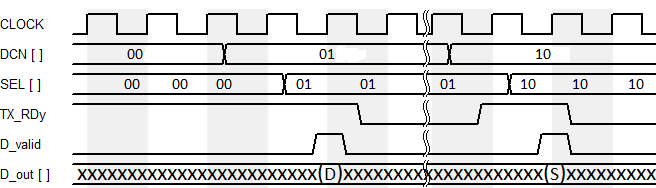
\includegraphics[width=1\textwidth]{timing_cu_mic.png}
    \caption{Timing del dato inviato}
    \label{fig:timing_small}
\end{figure}
Dalla figura è osservabile in maniera migliore come avviene l'invio del dato al trasmettitore, partendo dal segnale in uscita dal decisore, cioè il DCN, asserito su due bit. Questo viene mandato alla control unit, la quale, un colpo di clock dopo, manda al multiplexer il selettore, che assume un valore equivalente a quello del segnale DCN, cioè "00", "01", "10" o "11".\\Quindi una volta che il segnale di SEL ha girato il mux sulla codifica corretta, corrispondente alla direzione di provenienza dello schiocco rilevata, ed il segnale TX\_RDY, proveniente dal trasmettitore, risulta essere alto, cioè il trasmettitotre è libero per potergli inviare il dato di uscita, allora viene portato a livello logico 1 il segnale di D\_valid, per un colpo di clock. Ciò comporta ,un colpo di clock successivo, l'abbassamento del TX\_RDY, che sta ad indicare che il trasmettitore è occupato essendo già in trasmissione e quindi non gli può essere inviato nessun ulteriore dato finchè la trasmissione non termina e questo torna alto.\\Dal timing è osservabile come nel momento in cui in D\_valid viene attivato, si ha un immediato invio del dato in uscita, corrispondente alla codifica binaria delle lettere S,N e D del codice ASCII, come spiegato precedentemente.
\subsection{Tempistiche dati}
Per quanto riguarda le tempistiche con cui il dato D\_out viene inviato al trasmettitore e quanto la UART impiega a trasmettere il dato, è stato necessario fare degli studi per verificare che il dato D\_out non arrivasse prima che la UART finisse la trasmissione precedente.\\Quindi per dimostrare che effettivamente i tempi coincidessero sono stati compiuti i seguenti ragionamenti:
\begin{itemize}
    \item avendo una frequenza di clock di 25 MHz, ed una frequenza del PDM di 2 MHz,  è stata determinata la durata di un PDM in termini di numero di colpi di clock:
    \begin{center}
     1 PDM$=\frac{25 MHz}{2 MHz}=12,5$ colpi di clock ; 
    \end{center}
    Si é approssimato questo risultato a 13 bit;
   \item decimando di un fattore 50, e quindi prendendo un PDM ogni 50, allora i colpi di clock sono stati incrementati a 625, moltiplicando i 12,5 colpi di clock di un PDM per un fattore di 50. Questo é stato necessario in quanto si vogliono ricostruire dei dati PCM con frequenza 40 KHz;
   \item dato che i campioni utilizzati per il calcolo dell'energia sono 10, allora i 625 colpi di clock, computati al punto precedente, necessari per estrapolare un campione dal decimatore, sono stati moltiplicati per 10, arrivando ad un numero di 6250 colpi di clock, che convertiti nel dominio del tempo equivalgono a 250 $\mu$s;
   \item nel decisore poi sono state inglobate 4 energie per valutare se lo schiocco provenisse da destra o da sinistra. Quindi il tempo impiegato per il calcolo di un'energia è stato ulteriormente moltiplicato per quattro, ottenendo così, 1000 $\mu$s;
   \item in seguito, dal decisore è stato mandato un segnale DCN, che arrivando alla CU, ha stimolato il segnale del selettore del multiplexer, che va a selezionare la codifica del dato in uscita da inviare. Per attuare questo processo è stato impiegato un colpo di clock, ovvero 40 ns, che sommati al tempo precedente ha comportato un tempo totale, per la determinazione del dato da inviare, di 1040  $\mu$s;
   \item per quanto riguarda le tempistiche della UART, questa trasmette uno stream di 10 bit, di cui uno di idle, uno di start, poi la codifica del dato inviato ed un bit di stop. La durata di ciascun bit è risultata essere di 104  $\mu$s, quindi essendo i bit 10, il tempo totale per la trasmissione di un dato risulta essere 1040  $\mu$s;
   \item dai risultati temporali dei punti precedenti è evidente che le tempistiche per la computazione del dato da inviare alla UART e la durata della trasmissione di questa sono concordi, impiegando entrambi i processi 1040  $\mu$s. E' per questo che nell'interfacciamento tra multiplexer ed UART, non è stato necessaria l'aggiunta di nessun ulteriore componente.
\end{itemize}
\section{Simulazione ModelSim}
Per simulare il sistema é stato necessario fare due diverse acquisizioni tramite il software Audacity, in cui in una é stato registrato del rumore di fondo e nell'altra é stato acquisito uno schiocco di dita (entrambi di una lunghezza circa di 2 ms) in formato PCM con frequenza di campionamento pari a 44100 Hz.\\Tramite Matlab, una volta caricato il file, è stato eseguito un oversampling per portare il segnale a 2 MHz ed in seguito si é convertito in formato PDM sfruttando il seguente algoritmo:
\begin{verbatim}
        qe=0;
    for n=1:s
        
         if x(n) >= qe
            z(n)=1;
         else
            z(n)= -1;
         end
            qe=z(n) - x(n) + qe;
    end
\end{verbatim}
\textit{NB: "s" é la lunghezza in campioni del file audio}\\\\
In questo semplice algoritmo ad ogni step si confronta il corrispettivo coefficiente della sorgente audio con una soglia, che viene aggiornata alla fine del ciclo. Questa é incrementata ad ogni passo  con l'errore tra il dato convertito in PDM e il suo reale valore PCM. Le sequenze così ottenute sono state utilizzate per eseguire i vari test.\\
Quindi mediante ModelSim è stato simulato il progetto completo, in modo tale da poter osservare visivamente il comportamento dei segnali di principale interesse.\\
E' stato progettato un semplice testbench, in cui vengono generati localmente i segnali PDM per il canale destro e sinistro, i quali poi vengono messi insieme tramite un mux, così da far arrivare su un'unica linea allo snap detector il dato in formato doble data rate. La struttura implementata é visibile in Figura \ref{fig:testbench}.
\begin{figure}[H]
    \centering
    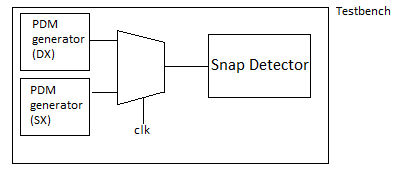
\includegraphics[scale=0.8]{testbench.png}
    \caption{Struttura del testbench}
    \label{fig:testbench}
\end{figure}
\noindent Successivamente sono riportate le varie simulazioni che sono state attuate, in cui il sistema implementato è stato connesso alla UART, così da compiere la trasmissione del dato desiderato.\\\\
In Figura \ref{fig:dx_sx} è riportata la prima simulazione.
\begin{figure}[H]
    \centering
    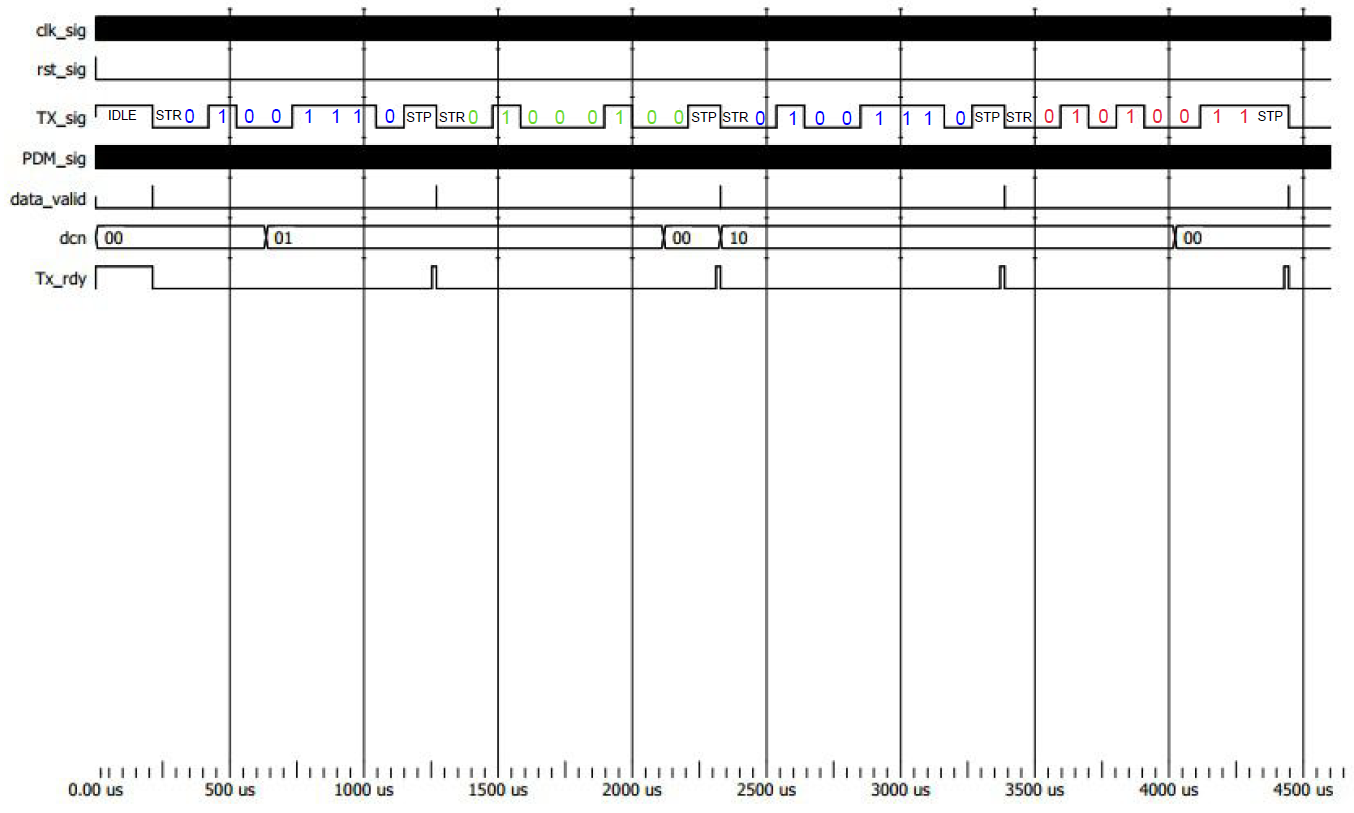
\includegraphics[width=1\textwidth]{dx_sx.PNG}
    \caption{Simulazione ModelSim trasmissione D ed S}
    \label{fig:dx_sx}
\end{figure}
\noindent La durata della simulazione è stata impostata a 4500 $\mu$s, in modo tale da poter vedere una completa trasmissione di tutte le casistiche possibili.\\Infatti dalla figura sopra riportata è possibile notale che inizialmente il trasmettitore è in uno stato di IDLE, essendo in quiete, senza star compiendo nessuna operazione, infatti il Tx\_rdy è impostato come alto, ovvero il trasmettitore è libero di ricevere un dato da inviare. Successivamente quando la prima decisione della provenienza dello schiocco è stata presa, il D\_valid è attivato per un colpo di clock. Ciò comporta quindi un abbassamento del Tx\_rdy e l'avvio della trasmissione del dato, riportato sul segnale TX.\\Su tale linea è infatti osservabile come dallo stato di IDLE, il sistemi passi a quello di START, indicato con l'abbreviazione "STR" e quindi inizi la trasmissione del dato inviato, codificato su 8 bit, susseguito dal bit di STOP, chiamato "STP" nell'immagine, che indica il termine della trasmissione. In seguito a questo infatti il Tx\_rdy tornerà alto, avendo completato la trasmissione.\\Dalla simulazione è visibile come tale segnale però torni subito basso, poichè, come già spiegato precedentemente nell'analisi delle tempistiche dell'arrivo dei dati, il sistema è stato progettato in modo tale che il momento in cui il trasmettitore finisce la trasmissione di un dato e quello in cui arriva un nuovo dato da inviare, siano coincidenti.\\Inoltre dai segnali rappresentati è possibile osservare che quando il decisore manda in uscita il DCN="00", il TX trasmette la codifica binaria della lettera N, data da "01001110", indicata dalla codifica in blu, la quale assume il significato dell'impossibilità di decretare una precisa provenienza dello schiocco. Mentre se DCN="01", la codifica sul segnale TX è "01000100", evidenziata dal colore verde, che corrisponde al codifica ASCII della lettera D, indicante che lo sciocco deriva da destra. Infine per un valore di DCN equivalente ad "10", sul TX è trasmessa la codifica corrispettiva alla lettera S, ovvero "01010011", riportata con il colore rosso, la quale comunica che lo schiocco è stato rilevato come proveniente da sinistra.\\\\Di seguito sono riportate altre due casistiche, che seguono una logica equivalente a quella descritta per la precedente simulazione. In Figura \ref{fig:dx_dx} è rappresentata la trasmissione prima del dato N ("01001110") e poi successivamente solo la D ("01000100"), che sta ad indicare che lo schiocco, inizialmente non percepito, poi viene rilevato sempre proveniente da destra.
\begin{figure}[H]
    \centering
    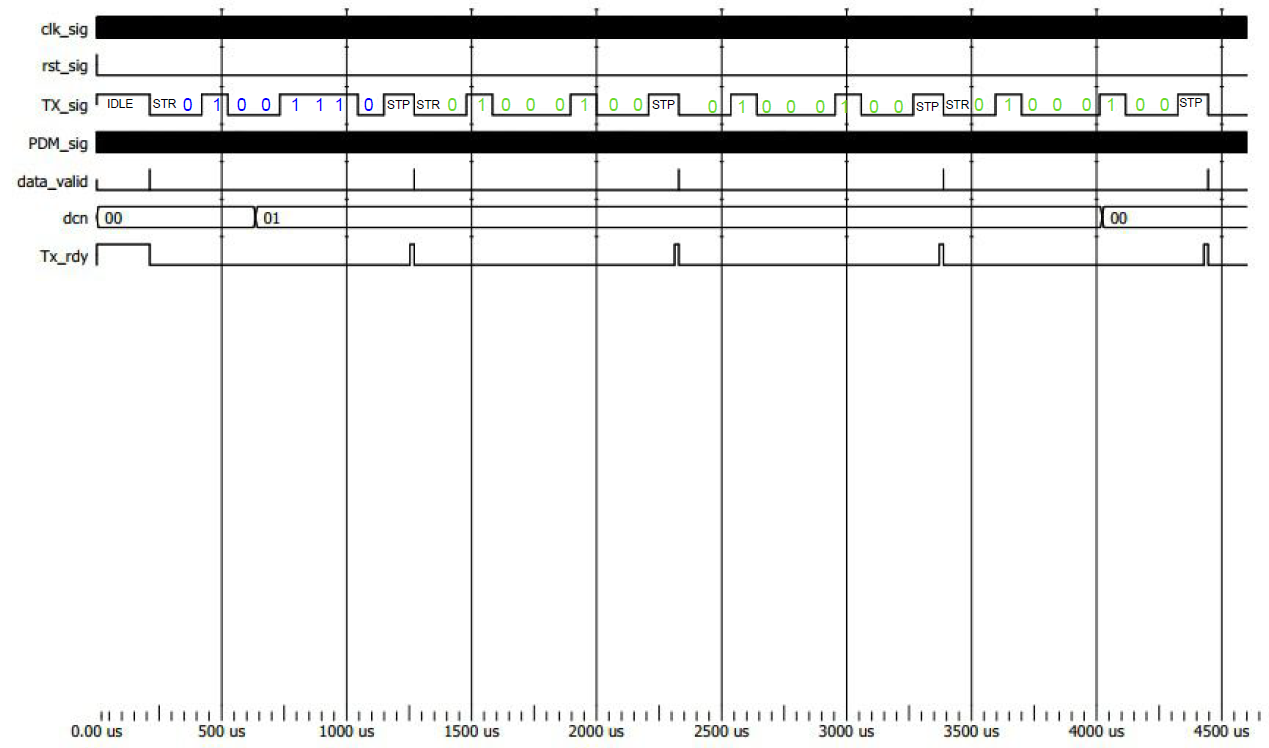
\includegraphics[width=1\textwidth]{dx_dx.PNG}
    \caption{Simulazione ModelSim trasmissione D}
    \label{fig:dx_dx}
\end{figure}
\noindent Mentre in Figura \ref{fig:sx_sx} è riportata la trasmissione inizialmente del dato nullo, per poi inviare sempre la codifica della lettera S ("01010011"), ovvero lo schiocco è derivante dalla parte sinistra rispetto alla posizione dei microfoni.
\begin{figure}[H]
    \centering
    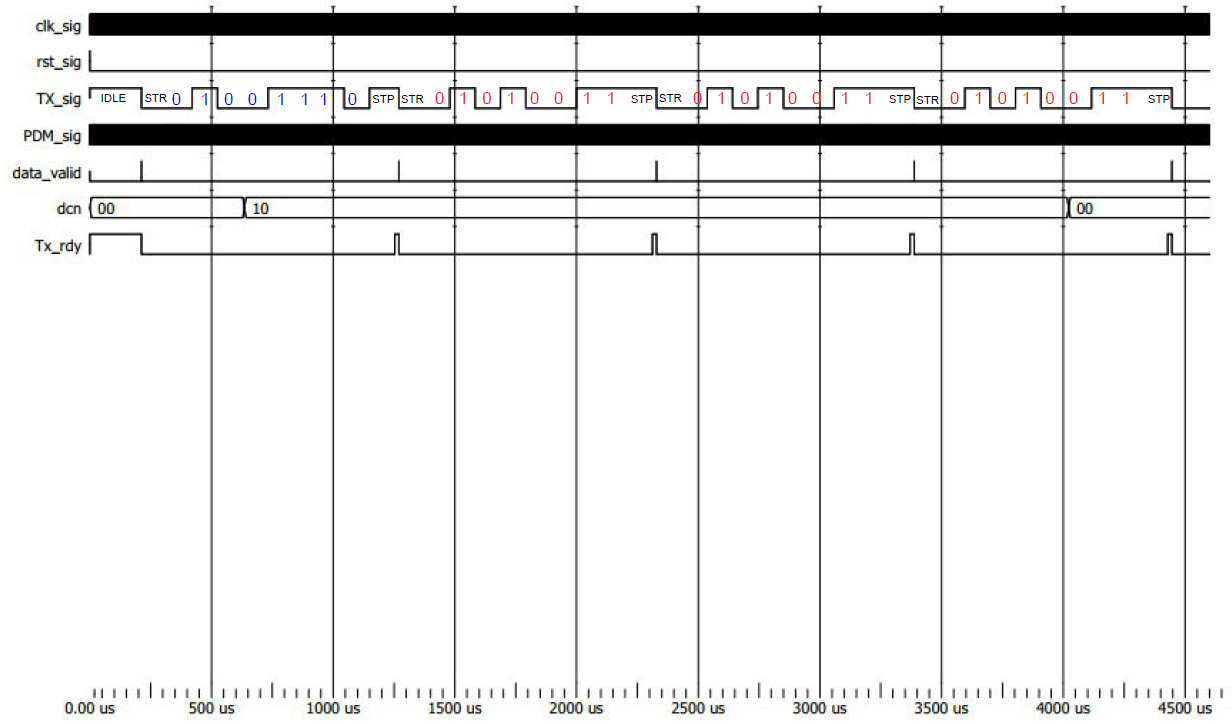
\includegraphics[width=1\textwidth]{sx_sx.PNG}
    \caption{Simulazione ModelSim trasmissione S}
    \label{fig:sx_sx}
\end{figure}
\subsubsection{Verifica tramite Matlab}
E' stato eseguito un ulteriore test per verificare che l'output PCM ricostruito dal sistema fosse congruente a quanto ottenuto per via teorica tramite le simulazioni eseguite su Matlab.
\newline
Lo schiocco acquisito tramite il microfono integrato del PC risulta essere nel tempo come in Figura \ref{fig:snap_acq}.\\Mentre in Figura \ref{fig:snap_per} é mostrato il periodogramma del segnale con le varie componenti in frequenza.

\begin{figure}[H]
    \centering
    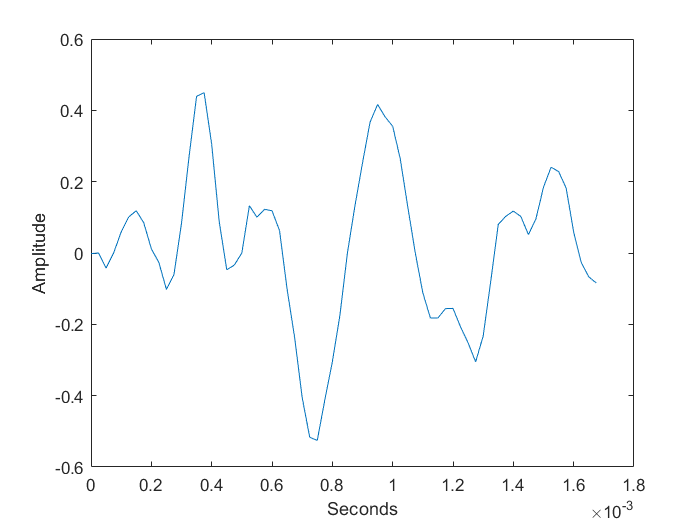
\includegraphics[scale=0.45]{sgn_camp.png}
    \caption{Schiocco acquisito}
    \label{fig:snap_acq}
\end{figure}

\begin{figure}[H]
    \centering
    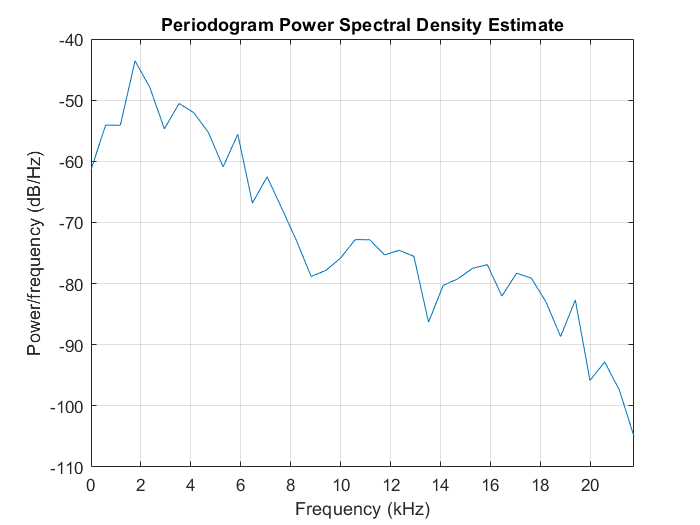
\includegraphics[scale=0.45]{spettr_camp.png}
    \caption{Periodogramma del segnale acquisito}
    \label{fig:snap_per}
\end{figure}

\noindent Dopo aver convertito la sorgente audio in PDM, questa in frequenza si presenta come in Figura \ref{fig:snap_per_PDM}. E' subito osservabile che la conversione ha spinto il rumore ad alte frequenze, come descritto in precedenza.
\begin{figure}[H]
    \centering
    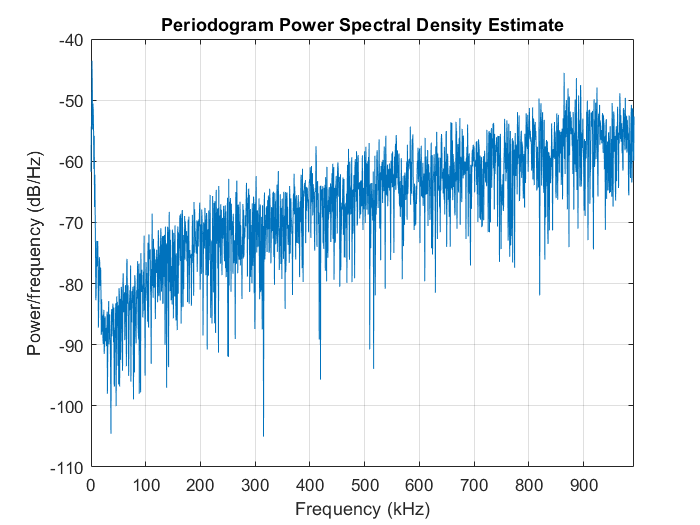
\includegraphics[scale=0.45]{spettr_PDM.png}
    \caption{Periodogramma del segnale PDM}
    \label{fig:snap_per_PDM}
\end{figure}
\noindent Applicando il filtro progettato, il segnale si presenta nel tempo come in Figura \ref{fig:snap_per_PDM_filt}, da cui è subito visibile come il segnale sia molto simile a quello di partenza.
\begin{figure}[H]
    \centering
    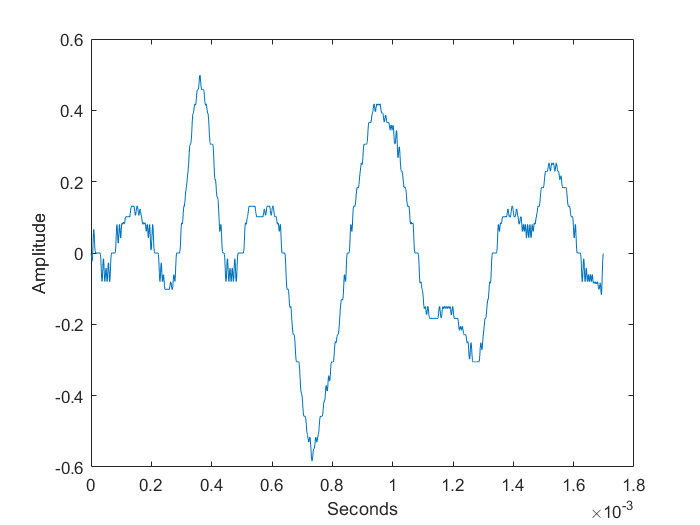
\includegraphics[scale=0.45]{filtered.png}
    \caption{Segnale PDM filtrato}
    \label{fig:snap_per_PDM_filt}
\end{figure}
\noindent Una volta filtrato, il segnale é stato sottocampionato per tornare a 40 kHz completando così la conversione in PCM. Quindi il segnale nel tempo viene rappresentato come in Figura \ref{fig:snap_PDM_filt_down} ed in frequenza (periodogramma) come in Figura \ref{fig:snap_per_PDM_filt_down}.
\begin{figure}[H]
    \centering
    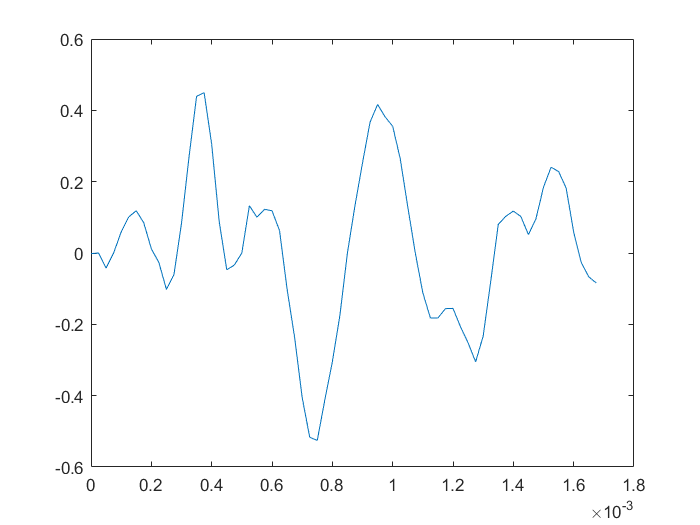
\includegraphics[scale=0.4]{filt_down.png}
    \caption{Segnale PCM ricostruito}
    \label{fig:snap_PDM_filt_down}
\end{figure}

\begin{figure}[H]
    \centering
    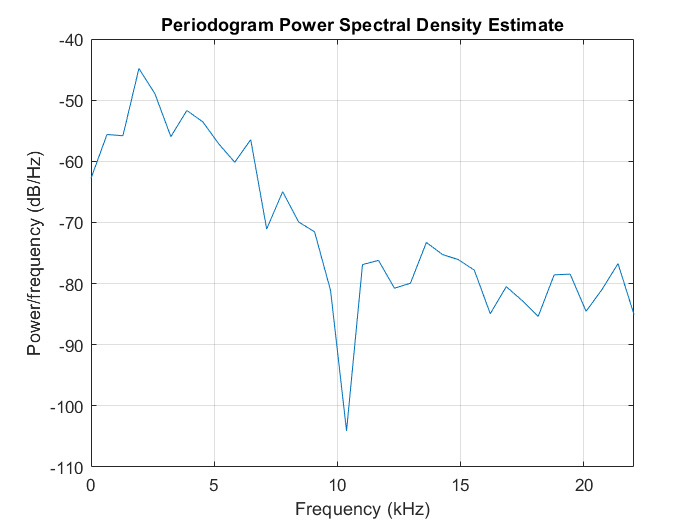
\includegraphics[scale=0.4]{filt_downt_period.png}
    \caption{Periodoframma segnale PCM ricostruito}
    \label{fig:snap_per_PDM_filt_down}
\end{figure}
\noindent Com'è possibile osservare, il processo di ricostruzione per via teorica é soddisfacente, infatti i due segnali sono molto simili, ed anche il periodogramma, a meno di qualche errore, segue un andamento molto vicino all'originario ed il picco si assesta su un livello simile di potenza rispetto all'originale.
\newline
Per verificare la bontà del sistema progettato sono stati acquisiti i dati in uscita dal decimatore dalle simulazioni Modelsim ed è stato ricostruito il segnale confrontandolo con l'originale.
\newline
Come è visibile in Figura \ref{fig:confronto} i segnali sono molto simili, attestando quindi che la conversione sia soddisfacente. Inoltre anche udendo il segnale ricostruito questo è risultato sembrare in tutto e per tutto uno schiocco (anche se per tale applicazione la qualità audio non é un parametro rilevante).
\begin{figure}[H]
    \centering
    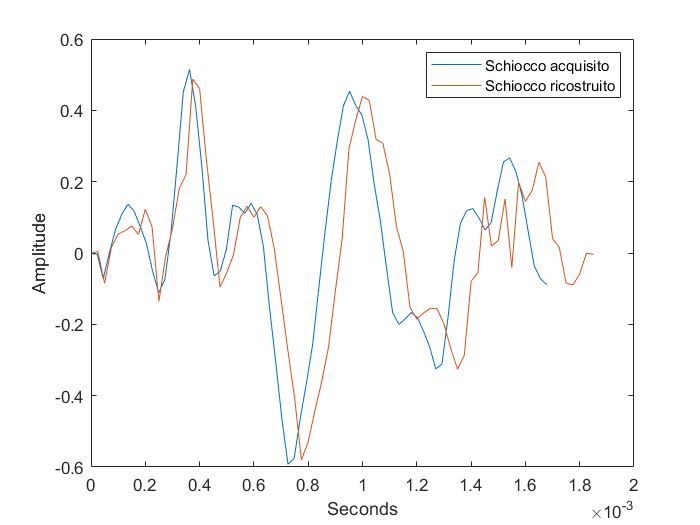
\includegraphics[scale=0.4]{confronto.png}
    \caption{Segnale ricostruito a confronto con l'originale}
    \label{fig:confronto}
\end{figure}
\noindent \textit{NB: Dalla figura é possibile notare un certo ritardo del segnale ricostruito, questo é dovuto all'operazione di filtraggio, che per un filtro FIR con N taps é pari a:
\begin{equation*}
  delay=\dfrac{N-1}{2  Fs} 
\end{equation*}}

\end{document}